\chapter{Projeto de implementação}
\label{cap:projetoimplementacao}

Neste capítulo será proposto uma solução de implementação de um ambiente de alta disponibilidade para os serviços críticos da empresa, que 
foram selecionados no capítulo anterior. Com isso pretende-se atingir o objetivo deste trabalho.

\section{Serviços críticos}
\label{section:servcrit}

No capítulo anterior foram detalhados todos os serviços que estão disponíveis na empresa. Nesta seção serão descritos os serviços que foram 
considerados mais críticos para a empresa. 

Para identificar quais são os serviços mais críticos para a empresa será definido alguns critérios, sendo assim os critérios são: 
\begin{itemize}
 \item A quantidade de clientes ou funcionários que utilizam o serviço: esse é o item mais relevante, pois impacta diretamente no faturamento
 da empresa. De fato, se um cliente ficar sem acesso à internet, o cliente terá um desconto proporcional ao tempo que ficou sem acesso; 
 \item O número de requisições em um determinado tempo: esse número é importante, uma vez que indicam a quantidade de usuários que dependem do 
 serviço. São exemplos dessa medida a quantidade de acessos por minuto em um servidor de hospedagens de sites e a quantidade de requisições 
 \ac{DNS} em um servidor recursivo;
 %\item O volume de elementos do serviço: essa medida demonstra a abrangência do serviço, ou seja, quantos objetos existem em um serviço.
 %Como por exemplo a quantidade de contas de \textit{e-mail} em um servidor de \textit{e-mail} e a quantidade de equipamentos monitorados por um 
 %servidor de monitoramento.
\end{itemize}

Considerando esses critérios, foram definidos que os serviços mais críticos são:
\begin{itemize}
 \item \ac{DNS} recursivo primário: esse serviço foi classificado como mais importante pois possui um impacto direto nos clientes do provedor. 
 Esse é o único serviço que todos os clientes e funcionários utilizam, sendo que os clientes são aproximadamente 9000. O objetivo de um provedor 
 é fornecer uma navegação de qualidade aos seus clientes, sendo assim, o \ac{DNS} é fundamental para essa navegação. Outro importante critério
 que pode ser aplicado ao \ac{DNS} recursivo é o número de requisições por segundo, que chega aproximadamente a 1150 (Figura \ref{fig:passata_day}),
 e assim esse serviço se torna o maior entre todos os outros;
 
\begin{figure}[h!]
 \centering
 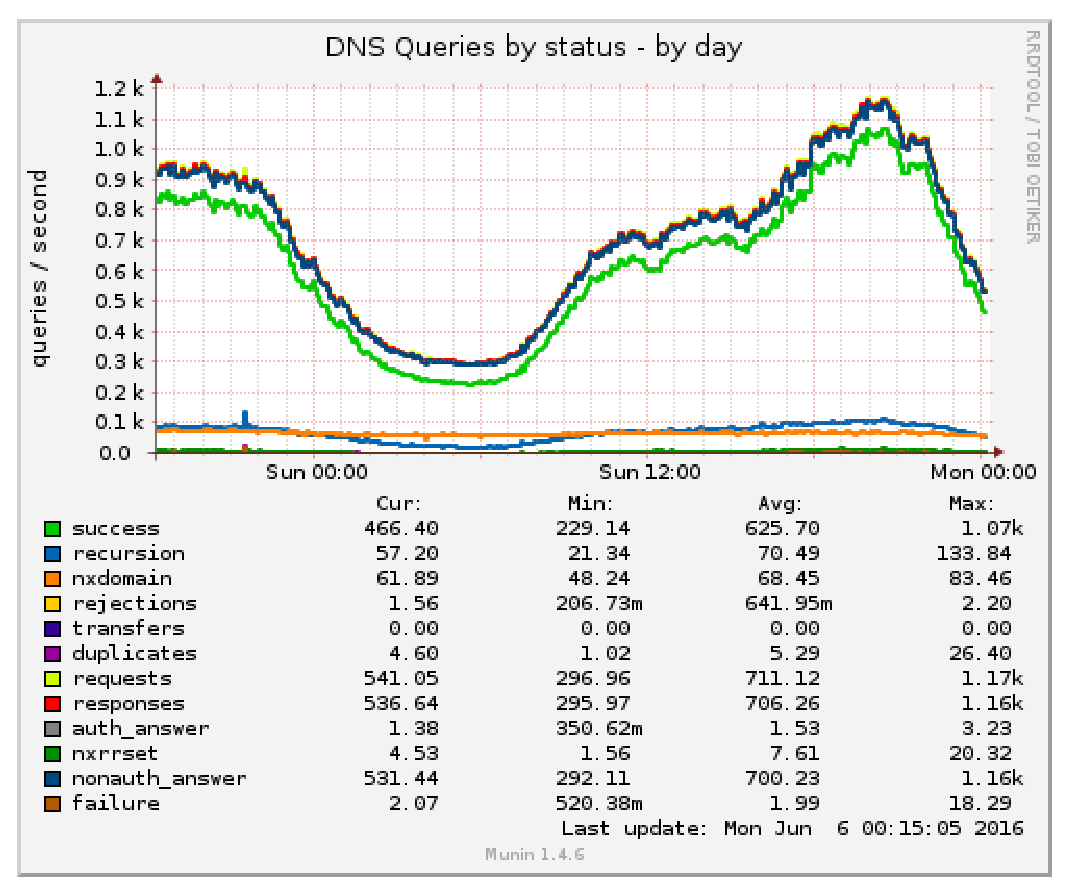
\includegraphics[width=310px]{img/passata_day.eps}
 \caption{Gráfico de requisições DNS.}
 \label{fig:passata_day}
\end{figure}

 \item \textit{Radius}: esse serviço também é importante para a navegação dos clientes do provedor, pois, ele faz a autenticação de todos os 
 clientes do provedor. Caso esse serviço fique indisponível os clientes não conseguirão estabelecer conexão para navegação. Esses servidores 
 recebem uma média de 1,6 requisições de autenticação por segundo (Figura \ref{fig:speedauth_auth_week} e \ref{fig:masterauth_auth_week}). 
 Além disso, esse serviço armazena dados importantes dos clientes para um provedor, que são os seguintes dados: o endereço de \ac{IP} de cada 
 cliente utilizado em um determinado período, o tráfego de dados da conexão, o tempo da conexão de cada cliente, o endereço \ac{MAC} dos 
 equipamentos dos clientes, entre outros. Essas operações resultam em um número de requisições por segundo, em média 23 requisições, que está 
 detalhado na Figura \ref{fig:speedauth_acct_week} e \ref{fig:masterauth_acct_week};
 
\begin{figure}[h!]
 \centering
 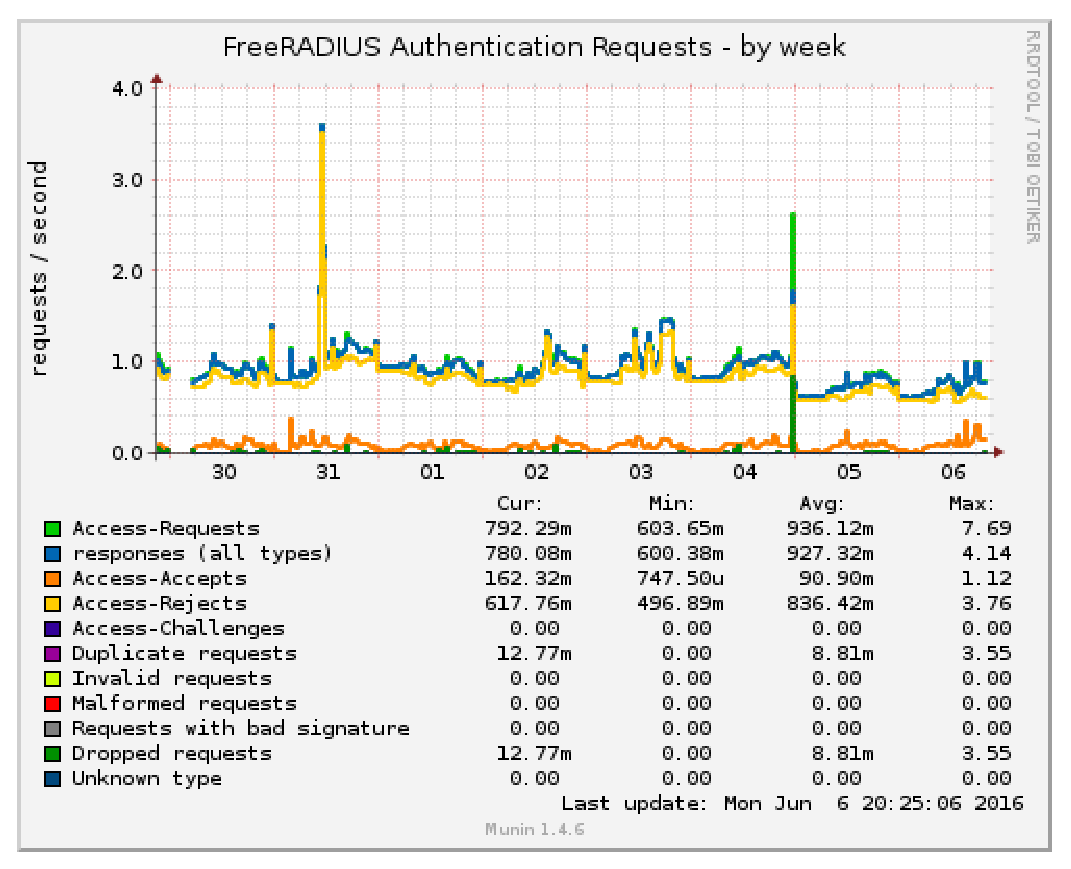
\includegraphics[width=310px]{img/speedauth_auth_week.eps}
 \caption{Gráfico de requisições de autenticação do servidor Speedauth.}
 \label{fig:speedauth_auth_week}
\end{figure}

\begin{figure}[h!]
 \centering
 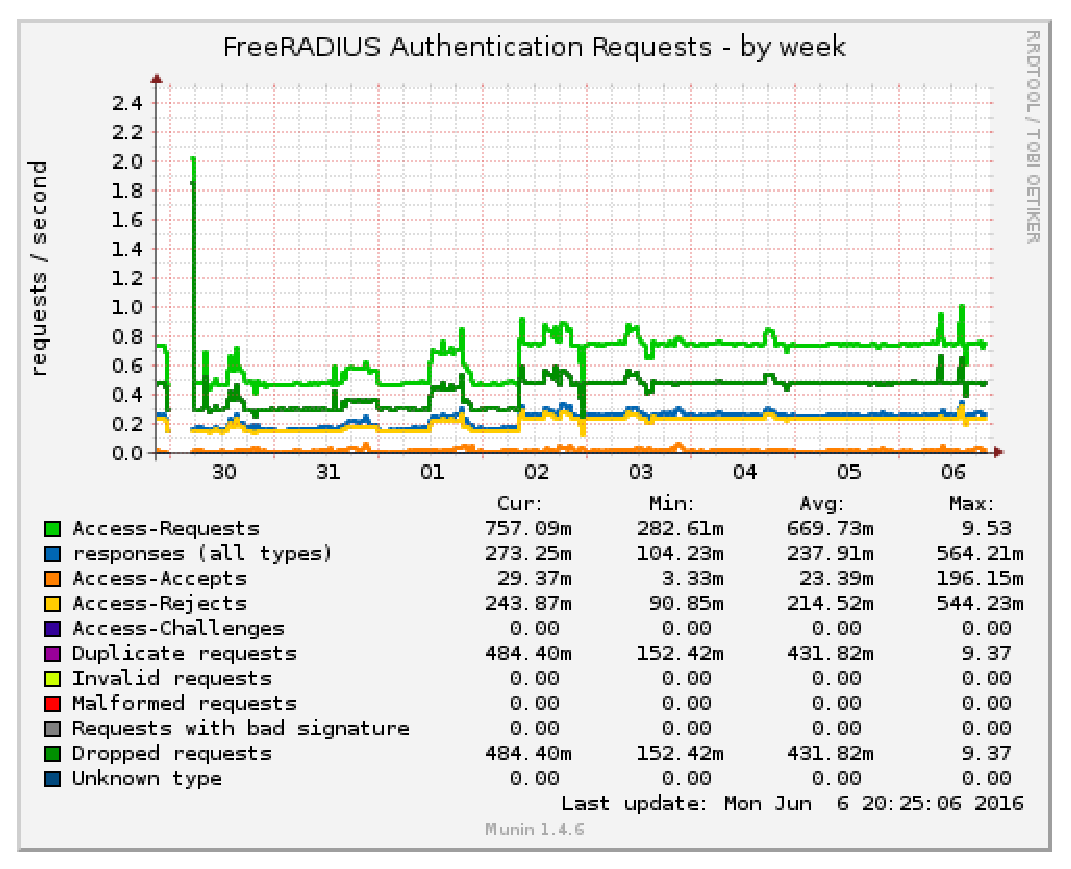
\includegraphics[width=310px]{img/masterauth_auth_week.eps}
 \caption{Gráfico de requisições de autenticação do servidor Masterauth.}
 \label{fig:masterauth_auth_week}
\end{figure}

\begin{figure}[h!]
 \centering
 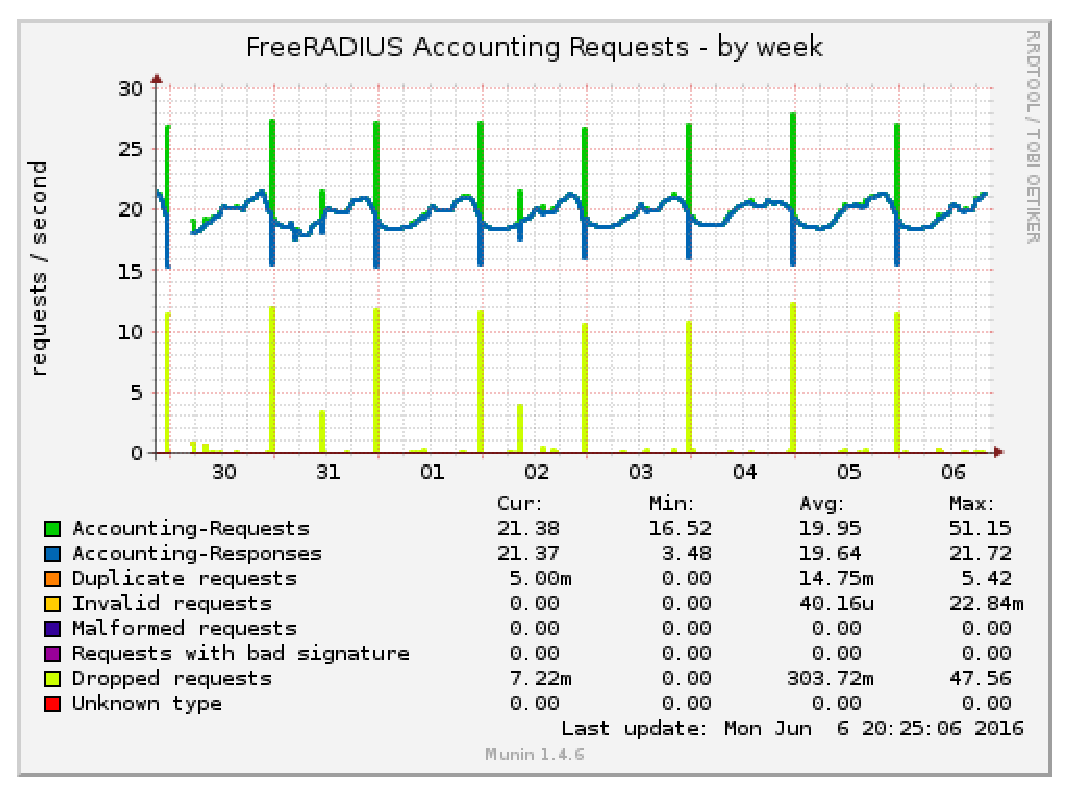
\includegraphics[width=310px]{img/speedauth_acct_week.eps}
 \caption{Gráfico de requisições de armazenamento do servidor Speedauth.}
 \label{fig:speedauth_acct_week}
\end{figure}

\begin{figure}[h!]
 \centering
 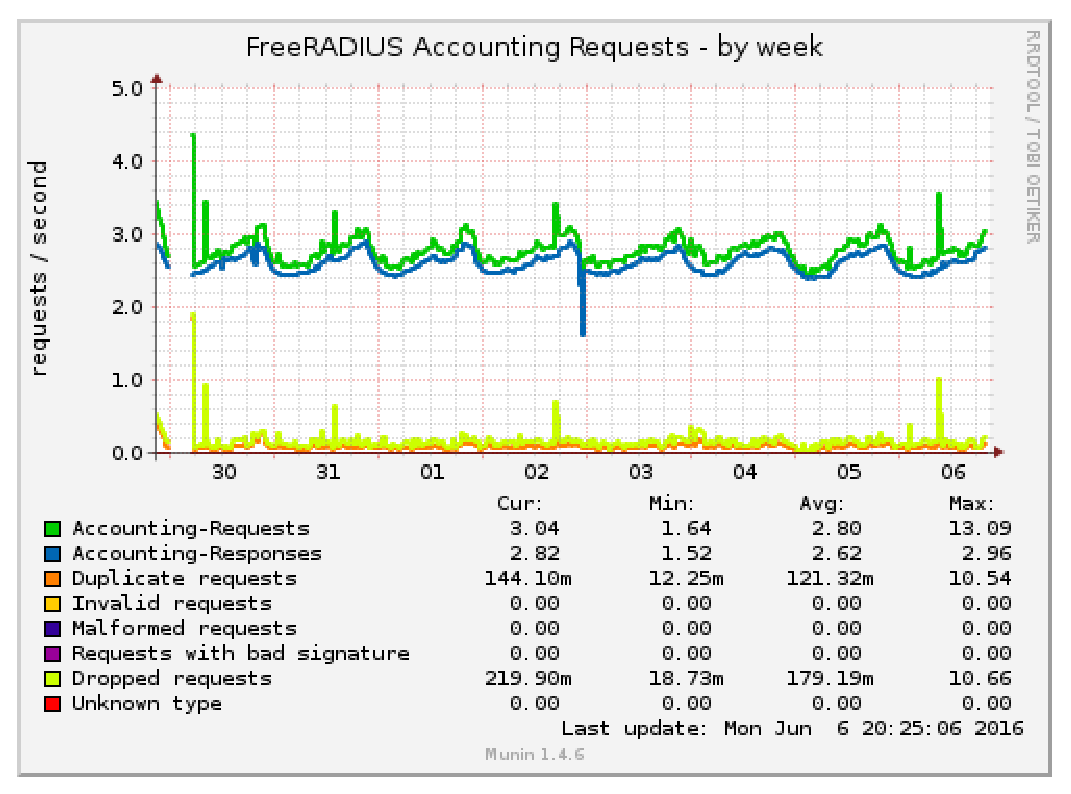
\includegraphics[width=310px]{img/masterauth_acct_week.eps}
 \caption{Gráfico de requisições de armazenamento do servidor Masterauth.}
 \label{fig:masterauth_acct_week}
\end{figure}

 \item Sistemas da empresa e do provedor: o sistema do provedor é responsável pela maior parte das operações do provedor, como por exemplo, 
 emissão de boletos e envio para clientes, atendimento de clientes, comunicação interna da empresa, vendas, ativações de novos clientes, entre 
 outros. Esse sistema não tem um grande impacto direto para os clientes, porém tem um grande impacto para os funcionários da empresa e do provedor. 
 Caso haja uma indisponibilidade dos sistemas a maior parte desses funcionários ficarão impossibilitados de trabalhar, sendo que são 
 aproximadamente 35 funcionários simultâneos (de acordo com a Figura \ref{fig:ejabberd_week}), isso poderia gerar um prejuizo elevado para a 
 empresa e o provedor. Outro critério que pode ser utilizando para esse serviço são as requisições por segundo recebidas pelo principal sistema 
 do provedor, essas chegam a aproximadamente 3 e 4 por segundo, conforme a Figura \ref{fig:soldi_week}. Além disso, a empresa mantém outros
 27 sistemas, de outros clientes, nesse mesmo servidor;
 
\begin{figure}[h!]
 \centering
 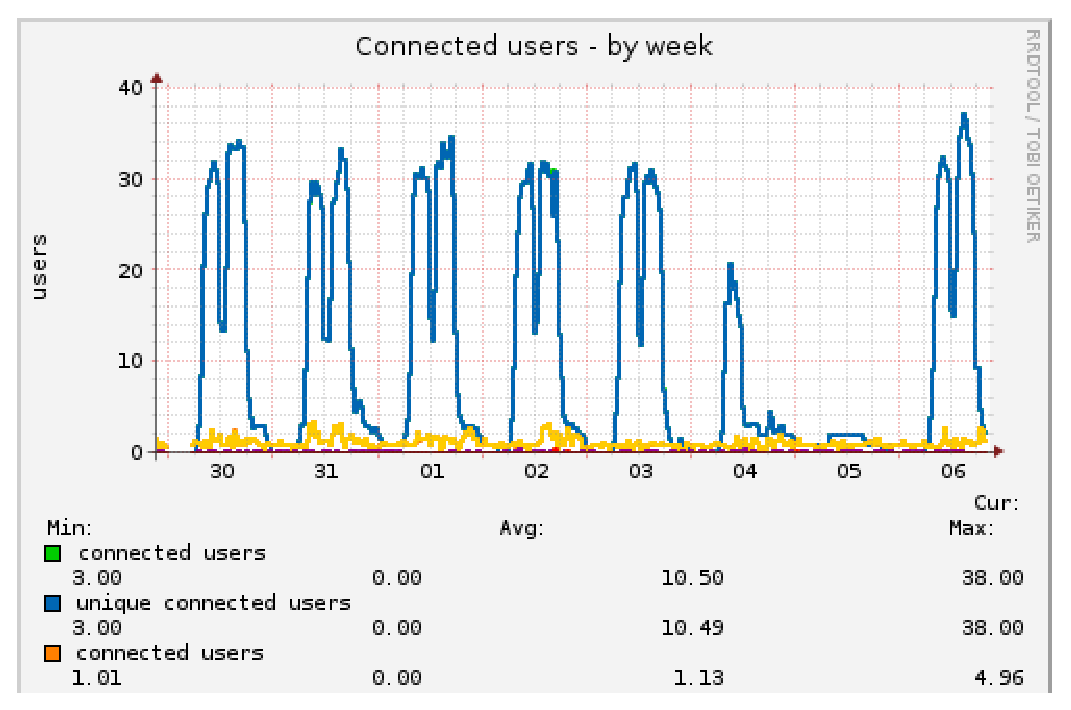
\includegraphics[width=310px]{img/ejabberd_week.eps}
 \caption{Gráfico usuários simultâneos de sistema.}
 \label{fig:ejabberd_week}
\end{figure}

\begin{figure}[h!]
 \centering
 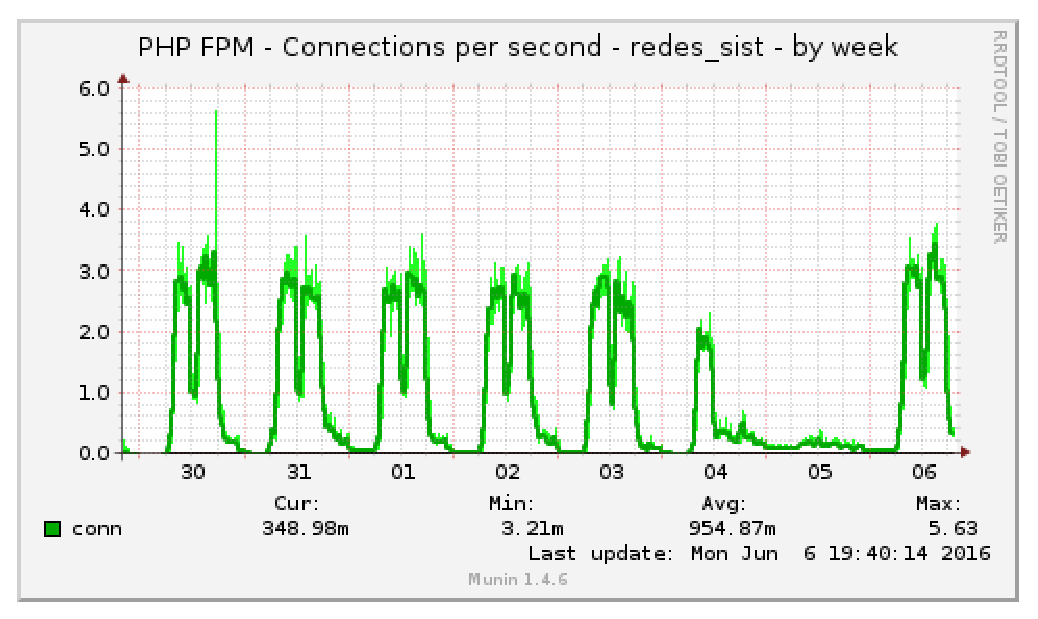
\includegraphics[width=310px]{img/soldi_week.eps}
 \caption{Gráfico de requisições por segundo do maior sistema.}
 \label{fig:soldi_week}
\end{figure}

 \item Telefonia: esse serviço tem relevância para a empresa e para o provedor, pois permite a comunicação entre clientes e funcionários, 
 e também entre funcionários e outros funcionários, sendo essencial para qualquer empresa. Exemplos desse serviço são: atendimento a clientes 
 para fins de suporte técnico, comunicação interna entre funcionários, comunicação com técnicos externos, cobranças a clientes inadimplentes, 
 vendas, entre outros. Levando isso em consideração, se esse serviço ficar indisponível irá gerar prejuízos para a empresa. 
 Para quantificar, no mês de maio de 2016 a empresa recebeu 15922 ligações, com duração total de 67 horas e 40 minutos, sendo que essas ligações 
 são feitas por todos os setores do provedor e também da empresa, além disso no mesmo mês foram efetuadas 674 ligações entre funcionários. 
 O gráfico da Figura \ref{fig:simplesip_week} mostra a quantidade de canais ativos simultaneamente no servidor de telefonia, com isso pode-se 
 perceber que existem de 20 e 30 ligações que são feitas durante o horário comercial.
\end{itemize}

\begin{figure}[h!]
 \centering
 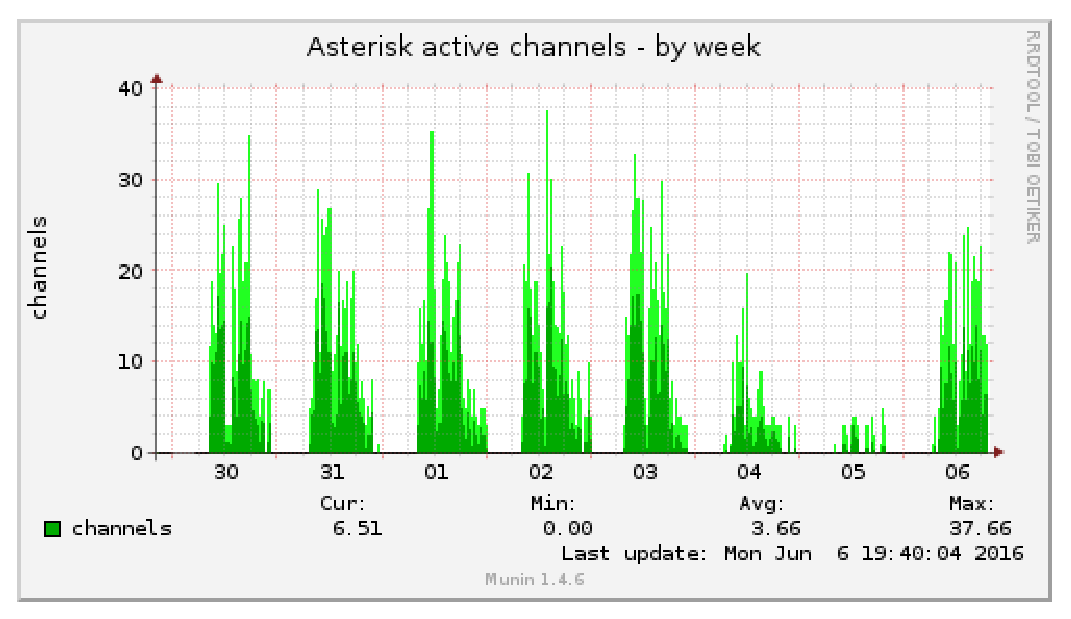
\includegraphics[width=310px]{img/simplesip_week.eps}
 \caption{Gráfico de requisições por segundo do maior sistema.}
 \label{fig:simplesip_week}
\end{figure}

Tendo esses serviços e os serviços mais utilizando, visto anteriormente, pode-se identificar quais máquinas virtuais deverão ser incluídas no 
ambiente de alta disponibilidade:
\begin{itemize}
 \item \textit{Passata}
 \item \textit{Speedauth}
 \item \textit{Masterauth}
 \item \textit{Soldi}
 \item \textit{SimplesIP}
\end{itemize}

Para selecionar os serviços mais utilizados pode-se compará-los utilizando algumas variáveis em comum para todos os servidores, que são o número 
de conexões \ac{TCP}, as transmissões \ac{UDP} e o número de elementos de cada serviço, esses elementos são por exemplo a quantidade de 
contas de \textit{e-mail} em um servidor de \textit{e-mail} ou a quantidade de equipamentos monitorados por um servidor de monitoramento. 
% Abaixo está a Tabela \ref{tab:servicoscompara} que possui os principais servidores e as variáveis:
% 
% %graficos fw_contrack e netstat
% \begin{table}[h!]
% \caption{Principais servidores comparados.}
% \label{tab:servicoscompara}
% \begin{center}
% \begin{tabular}{|p{2cm}|l|l|l|}\hline
% Servidor & Elementos & Conexões TCP & Transmissões UDP\\\hline
% Masterauth & 966 & 101 & 80\\\hline
% Merak & 1727 & 50,7 & 0\\\hline
% Ns & 358 & 1,02 & 1940?\\\hline
% Passata & 0 & 1,19 & 23430\\\hline
% Rauco & 109 & 12,87 & 0\\\hline
% Roncon & 122 & 5,78 & 0\\\hline
% SimplesIP & 36 & 41,11 & ?\\\hline
% Soldi & 27 & 36,16 & 278,66\\\hline
% Speedauth & 7878 & 51,02 & 653,36\\\hline
% \end{tabular}
% \end{center}
% \end{table}

O gráfico da Figura \ref{fig:servico_tcp} demonstra que os servidores que estabelecem mais conexões \ac{TCP} são o \textit{Speedauth} e o 
\textit{Masterauth}, também pode-se perceber que os servidores \textit{Merak}, \textit{SimplesIP} e \textit{Soldi} possuem um número considerável 
de conexões. Por outro lado, com o gráfico da Figura \ref{fig:servico_udp} pode-se perceber que o servidor \textit{Passata} possui um
número elevado de transmissões \ac{UDP} comparado aos outros, entretanto, o servidor \textit{SimplesIP} possui o segundo maior número. Já a Figura 
\ref{fig:servico_elemento} demonstra que o servidor \textit{Speedauth} possui um número alto de elementos, assim o destacando dos outros servidores.
Sendo assim, pode-se fazer uma análise dos três gráficos anteriores e concluir que os servidores \textit{Passata}, \textit{Speedauth}, 
\textit{Masterauth}, \textit{Soldi} e \textit{SimplesIP} são os servidores mais utilizados por clientes e funcionários.

\begin{figure}[h!]
 \centering
 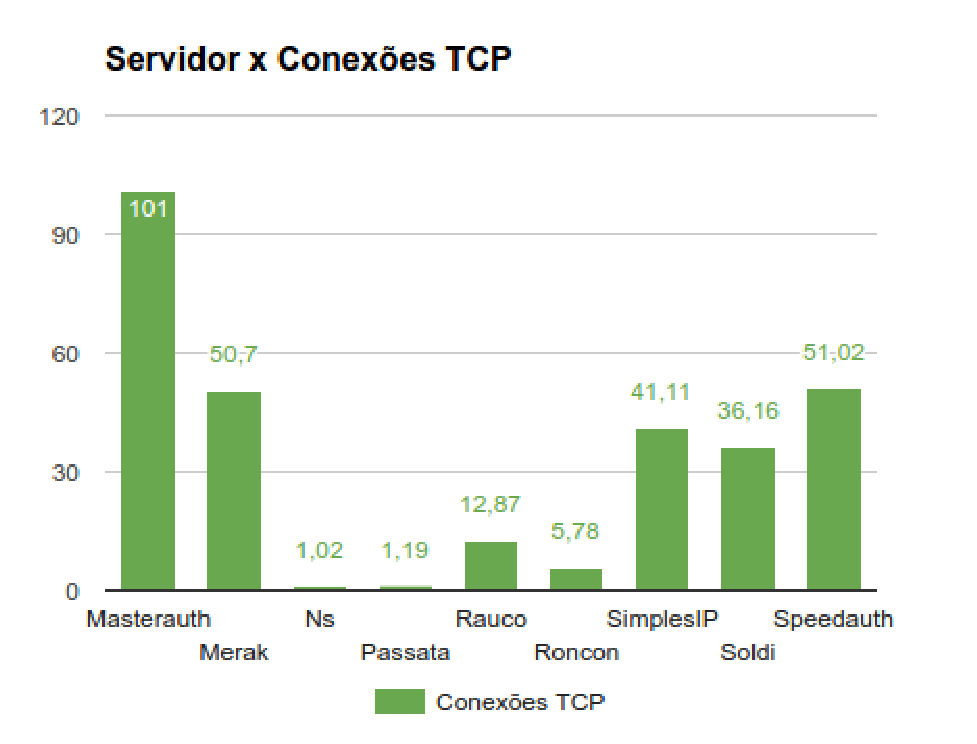
\includegraphics[width=280px]{img/servico_tcp.eps}
 \caption{Gráfico de comparação de conexões TCP entre os principais servidores.}
 \label{fig:servico_tcp}
\end{figure}

\begin{figure}[h!]
 \centering
 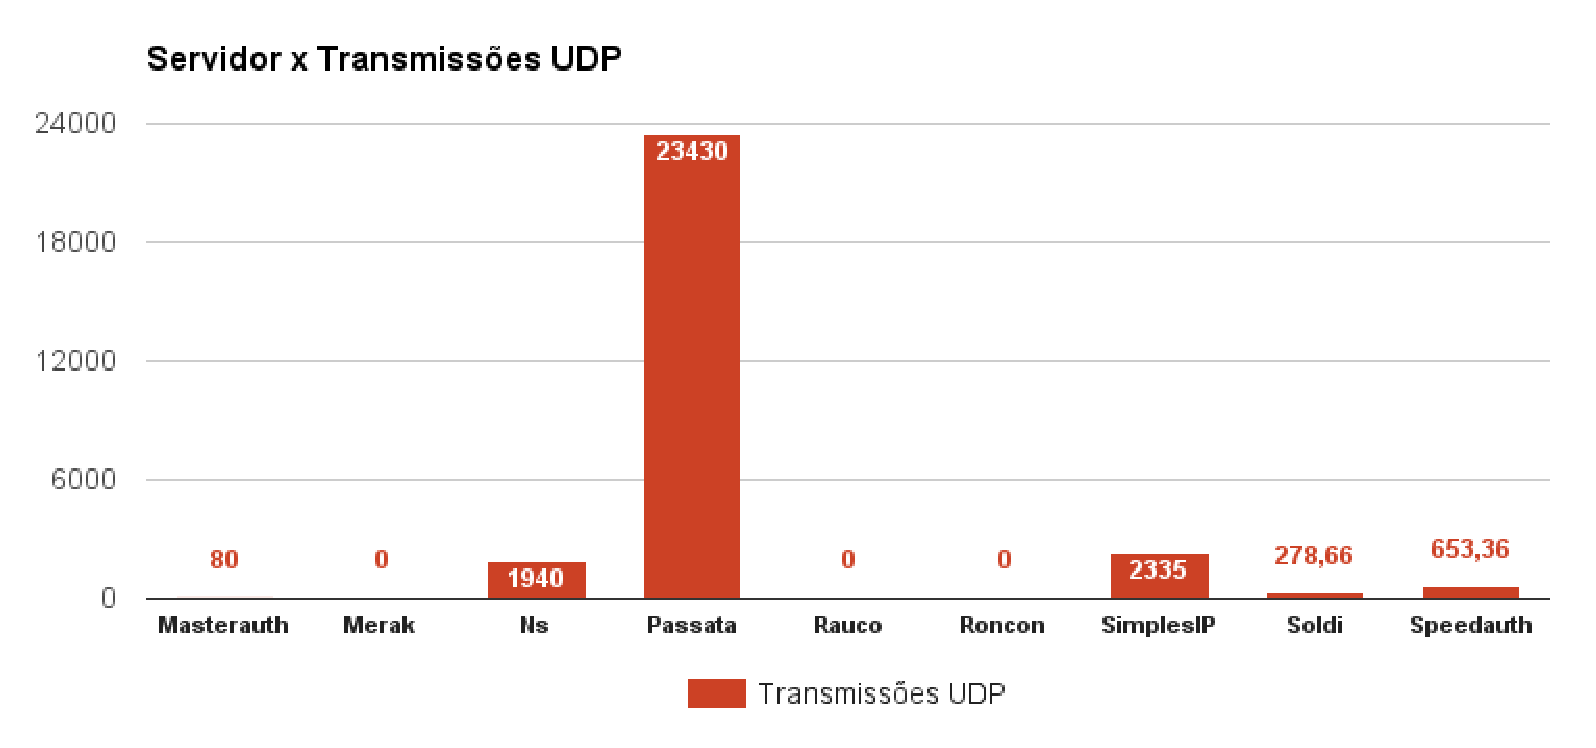
\includegraphics[width=280px]{img/servico_udp.eps}
 \caption{Gráfico de comparação de transmissões UDP entre os principais servidores.}
 \label{fig:servico_udp}
\end{figure}

\begin{figure}[h!]
 \centering
 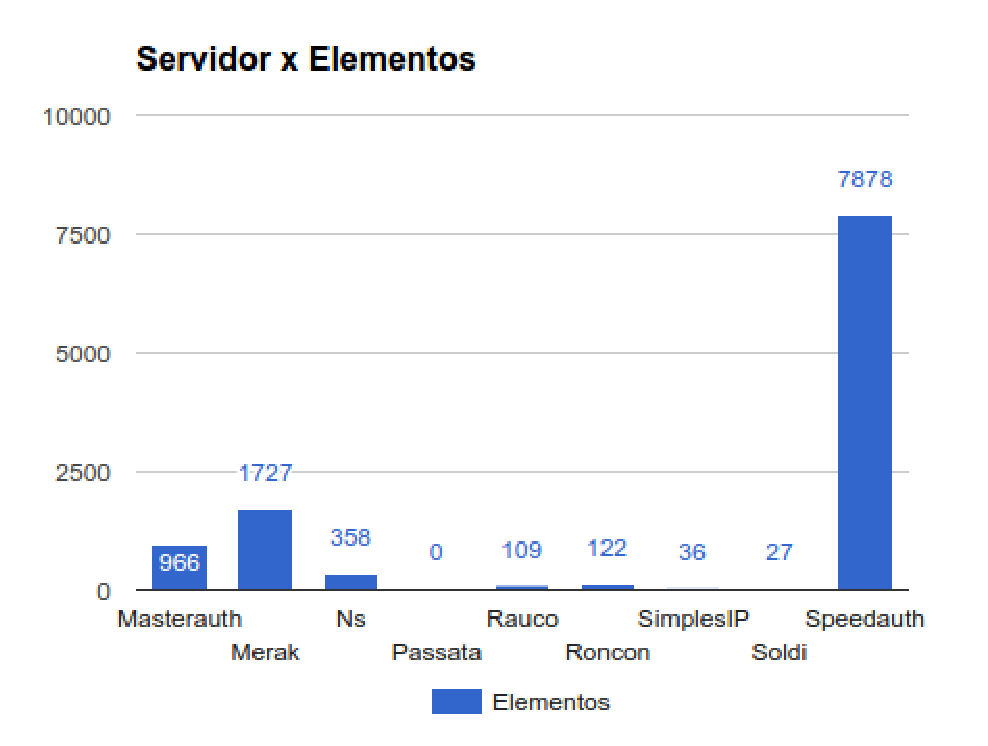
\includegraphics[width=280px]{img/servico_elemento.eps}
 \caption{Gráfico de comparação de elementos entre os principais servidores.}
 \label{fig:servico_elemento}
\end{figure}


\section{Proposta de solução}

O primeiro passo desta implementação é fazer uma reorganização das máquinas virtuais entre os servidores atuais, liberando assim o 
\textit{hardware} suficiente para possibilitar a implementação do ambiente de alta disponibilidade. 

Após ter sido feito a reorganização das máquinas virtuais será iniciado a implementação, montando um ambiente com dois servidores e os 
configurando de uma forma que caso houver alguma falha, em um servidor físico ou no seu sistema operacional hospedeiro, as máquinas serão 
tranferidas para o outro servidor físico. 
A configuração dos servidores deverá ser de 11 \textit{cores} de processamento, 12 GB de memória e 156 GB de disco, sendo que essa configuração 
foi calculada a partir da soma dos recursos atuais das máquinas virtuais que possuem os serviços críticos, que foram apresentadas no capítulo
anterior na Seção \ref{section:servcrit}.

As ferramentas necessárias para essa implementação podem ser divididas em dois grupos: ferramenta de replicação de dados 
(Seção \ref{section:toolrepl}) e ferramenta que faz o monitoramento e a tranferências das máquinas virtuais no caso de alguma falha 
(Seção \ref{section:toolcluster}).

\section{Ferramentas de replicação de dados}
\label{section:toolrepl}

Replicação de dados pode ser feita de diversas maneiras, pode ser a nível de aplicação ou até mesmo a nível de \textit{hardware}.
Dependendo do objetivo e da aplicação pode-se usar ferramentas como por exemplo o \textit{rsync}, que faz o sincronismo de dados de uma origem
para um destino. Sendo assim, não é possível utilizar essa ferramenta, pois ela não faz a replicação em tempo real, ou seja, se for necessário
utilizar os dados de destino ocorrerá perda de dados devido ao tempo de sincronismo. Outra forma de replicação é a de discos com \ac{RAID} 
por exemplo, essa solução é eficaz para garantir que o sistema não fique indisponível em caso de falha de discos\footnote{Lembrando que essa 
solução é utilizada no ambiente atual para aumentar a disponibilidade dos servidores}, porém não garante a disponibilidade quando \textit{software}
ou algum outro componente de \textit{hardware} falhar \cite{zaminhani2008}.

A solução de replicação ideal para esta implementação é um espelhamento de dados através da redes, sendo que essa solução permite a cópia dos 
dados para uma máquina remota em tempo real. Essa solução além de fazer a replicação dos dados, faz a redundância de todo \textit{hardware}.

A ferramenta escolhida para replicação de dados na solução de alta disponibilidade desse trabalho foi o \ac{DRBD}. Essa ferramenta é de código
aberto, e permite a replicação de dados de um dispositivo local em tempo real. 
APROFUNDAR AQUI OU NA IMPLEMENTAÇÂO? AQUI

figura??

% dispositivo primario e secundario zaminhani2008
% Segundo (ELLENBERG, 2007), a partir da versão 8 do DRBD é possível que,
%dependendo da aplicação, a execução ocorra em todos os nós do cluster
%simultaneamente (Ativo/Ativo). Para tornar isso possível é necessária a
%utilização de um sistema de arquivos exclusivo para cluster, como o OCFS2 6 e o
%GFS 7 por exemplo. Como a abordagem deste trabalho é cluster de alta
%disponibilidade, a utilização do DRBD no modo Ativo/Ativo não será discutida.

\section{Ferramentas de gerenciamento de cluster}
\label{section:toolcluster}

Para ser possível implementar uma solução de alta disponibilidade é necessário uma ferramenta que monitora os recursos, fazendo a detecção e
recuperação do serviço utilizando mensagens entre os servidores, que é denominada como um \textit{cluster} \cite{perkov2011}. 
Pode-se definir \textit{cluster} como um grupo de computadores interligador por rede com o objetivo de aumentar o desempenho ou disponibilidade
de um serviço \cite{freitas2005}.

Essas ferramentas de gerenciamento de \textit{cluster} permitem detecção de falhas a nível de nó e a nível de recursos, ou seja, pode detectar
falhas de \textit{hardware} e falhas de serviços (recursos).
Elas são conhecidas como \ac{CRM}, cujo sua função é fazer a gerência de recursos de um \textit{cluster}.

O \ac{CRM} escolhido para gerenciar o ambiente foi o \textit{Pacemaker} ...
Outras ferramentas CRM:
Microsoft com+ cluster ???
ZS3-2 Clustering ???

O \textit{Pacemaker} \cite{pacemaker}, que pode ser definido como uma ferramenta de detecção e recuperação de falhas a nível de 
serviço \cite{perkov2011}. Essa ferramenta é um projeto de código aberto mantido pela \cite{clusterlabs}, e teve origem com a necessidade de 
criar um gerenciador de recursos para a ferramenta \textit{Heartbeat} \cite{heartbeat}. 

O \ac{CRM} \textit{Pacemaker} possui algumas características que estão listadas abaixo:
\begin{itemize}
 \item Inicia e para serviços;
 \item Replica a configuração do \textit{cluster} para todos os nós de forma transparente, com isso a configuração de todo o \textit{cluster} pode ser feita em qualquer nó;
 \item ...
\end{itemize}

A arquitetura do \textit{Pacemaker} pode ser dividida em três partes:
\begin{itemize}
 \item 
\end{itemize}

Esse \ac{CRM} funciona em conjunto com ferramentas de troca de mensagens ...

\begin{figure}[h!]
 \centering
 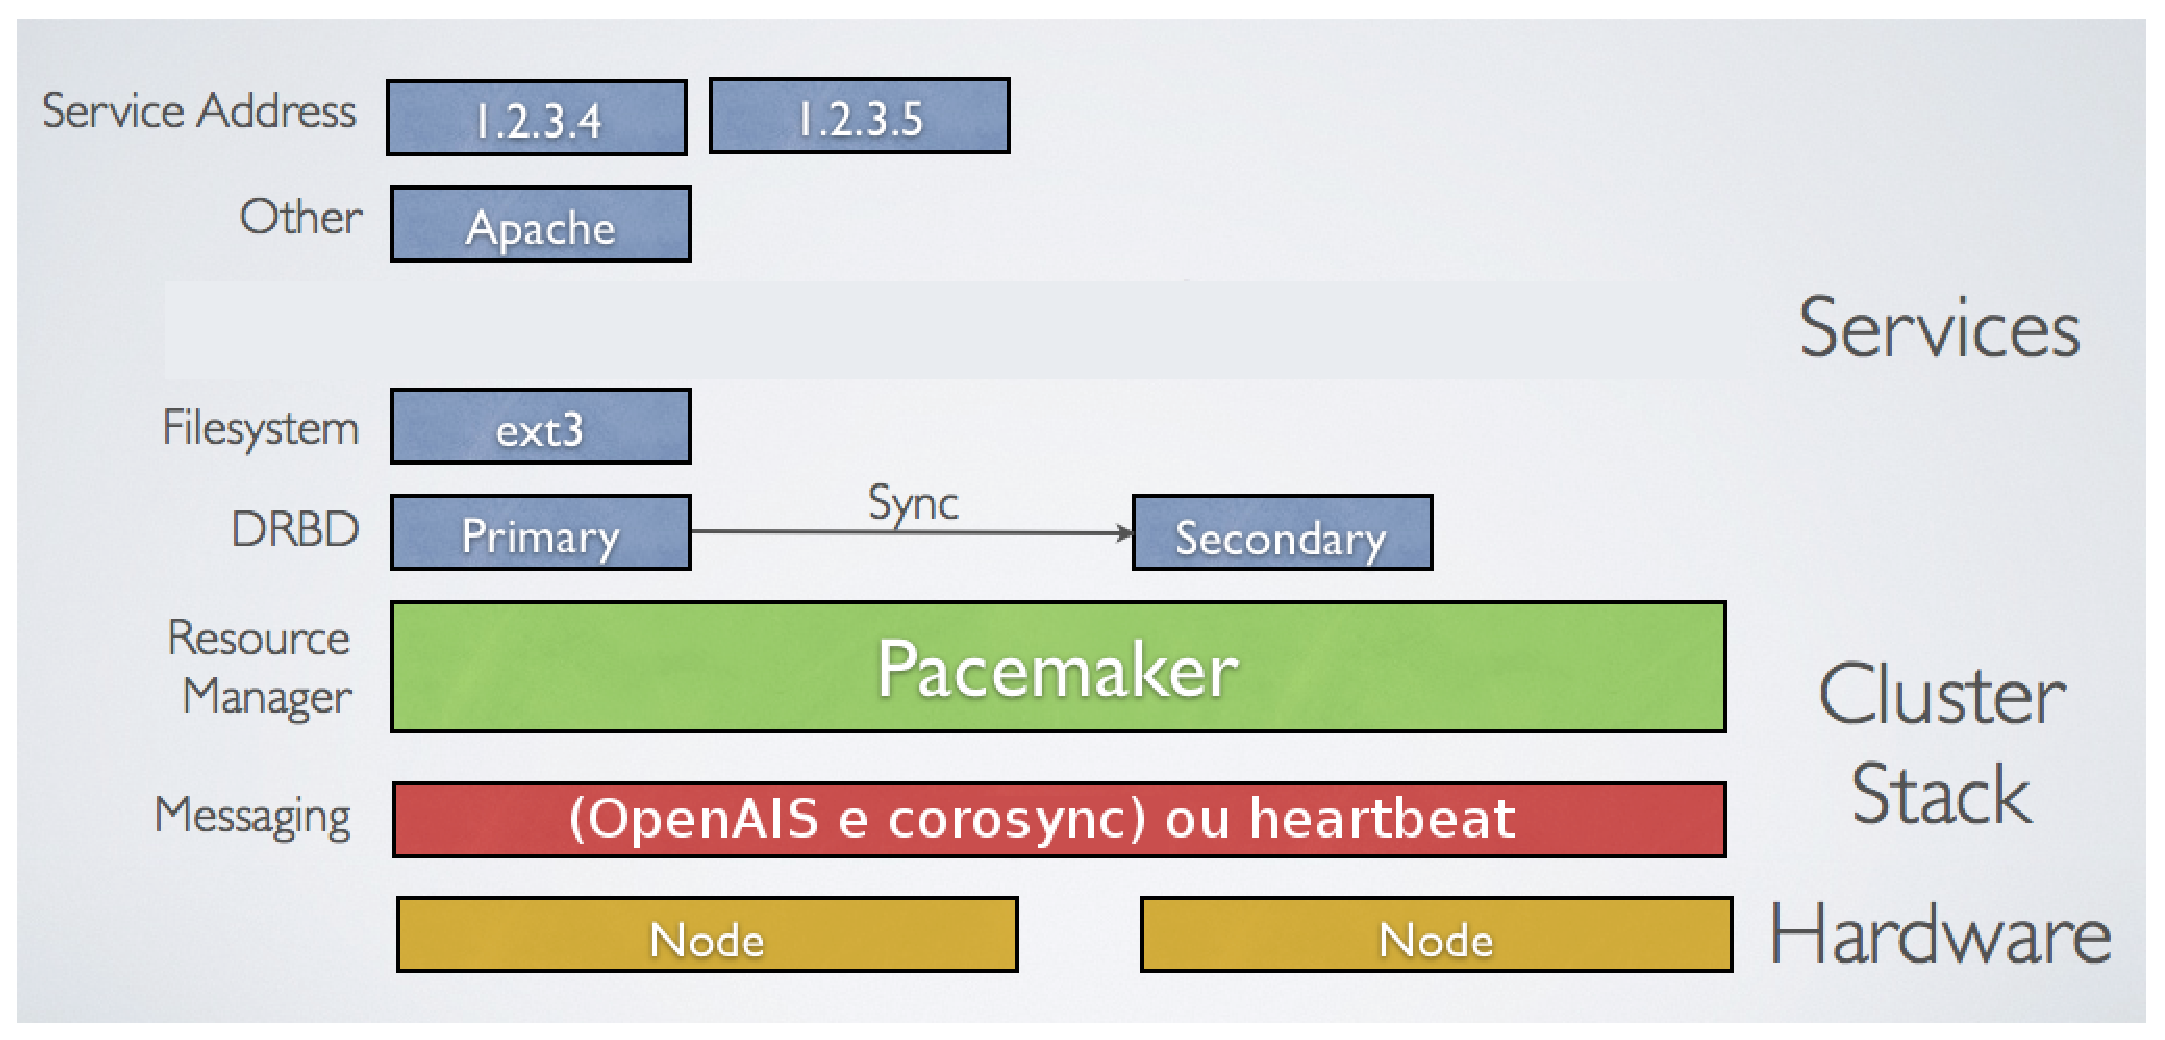
\includegraphics[width=300px]{img/pacemaker_tools.eps}
 \caption{Pacemaker estrutura}
 Fonte: \citet{pacemaker}
 \label{fig:pacemaker_tools}
\end{figure}

O \textit{Heartbeat} é um mecanismo que faz envio de mensagens entre os nós do \textit{cluster} com objetivo de notificar esse 
\textit{cluster} quando houver alguma alteração de estado dos recursos ou dos nós \cite{clusterlabs}. O \textit{Heartbeat} é um subprojeto do
\textit{Linux-HA} \cite{linuxha}.

As ferramentas \textit{OpenAIS} e \textit{Corosync} ...

\cite{clusterlabs}:
Corosync provides pacemaker:
a mechanism to reliably send messages between nodes,
notifications when machines appear and disappear
a list of machines that are up that is consistent throughout the cluster 
Heartbeat provides:
a mechanism to reliably send messages between nodes,
notifications when machines appear and disappear
a list of machines that are up that is consistent throughout the cluster 
--
http://serverfault.com/questions/269831/relation-between-heartbeat-openais-corosync
well i reached answer on myself! clustering include two part:
1.cluster resource management
2.infrastructure with massaging layer
legacy heartbeat is broken into heartbeat message layer and pacemaker so pacemaker is CRM.
and we have two option on message layer:heartbeat,openais. openais/corosync is preferred as: http://comments.gmane.org/gmane.linux.highavailability.user/32355
There are, however, features in Pacemaker that require OpenAIS which will work only with Corosync, not Heartbeat. Those features are concerned 
with the distributed lock managers used by cLVM (but not regular LVM), GFS/GFS2, and OCFS2. If you need that functionality, you must select 
OpenAIS/Corosync. If you do not, you're free to choose.
as: http://www.clusterlabs.org/wiki/FAQ
Originally Corosync and OpenAIS were the same thing. Then they split into two parts... the core messaging and membership capabilities are now 
called Corosync, and OpenAIS retained the layer containing the implementation of the AIS standard.
Pacemaker itself only needs the Corosync piece in order to function, however some of the applications it can manage (such as OCFS2 and GFS2) 
require the OpenAIS layer as well.
so i went to openais/corosync and integrate it with pacemaker.
--
There are, however, features in Pacemaker that require OpenAIS which
will work only with Corosync, not Heartbeat. Those features are
concerned with the distributed lock managers used by cLVM (but not
regular LVM), GFS/GFS2, and OCFS2. If you need that functionality, you
must select OpenAIS/Corosync.

Pacemaker itself only needs the Corosync piece in order to function, however some of the applications it can manage 
(such as OCFS2 and GFS2) require the OpenAIS layer as well. 

cluster resource manager (CRM) which has the task of starting and stopping the services (IP addresses, web servers, etc)


Explicar live migration \ref{fig:vms_migration}
%http://www.aliancatecnologia.com/conteudo/2015/05/quatro-estrategias-de-protecao-para-seu-ambiente-virtual/

\begin{figure}[h!]
 \centering
 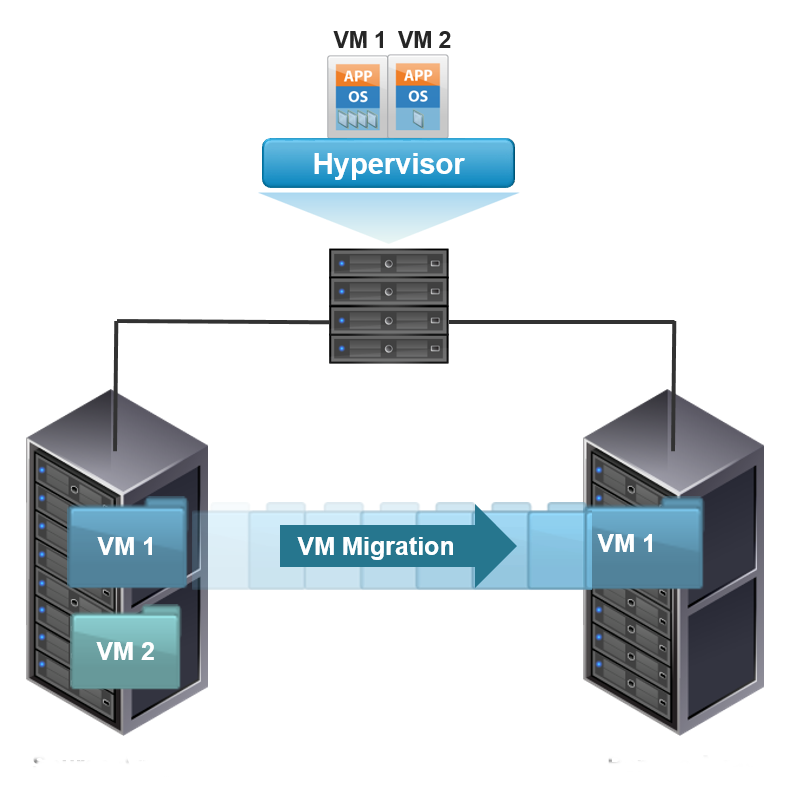
\includegraphics[width=300px]{img/vms_migration.eps}
 \caption{Live migration}
 Fonte: \citet{spaniol2015}
 \label{fig:vms_migration}
\end{figure}


%reorganização de vms
%ferramentas selecionadas, colocar motivo para escolher e citar ferramentas parecidas
%muitos servicos, melhor solucao utilizar 2 servidores para fazer redundancia
%em caso de falha de um servidor fisico...
%ferramentas open source...
%colocar a disponibilidade do nagios do ano passado?
